%%%%%%%%%%%%%%%%%%%%%%%%%%%%%%%%%%%%%%%%%%%%%%%%%%%%%%%%%%%%%%%%%%%%%%%%%%%%%%%%%%%%%%%%%%%%%%
% Template Beamer Sugestivo para Projetos no Senac
% by ezefranca.com
% Based on MIT Beamer Template
% As cores laranja e azul seguem o padrao proposto no manual de uso da identidade visual senac
%%%%%%%%%%%%%%%%%%%%%%%%%%%%%%%%%%%%%%%%%%%%%%%%%%%%%%%%%%%%%%%%%%%%%%%%%%%%%%%%%%%%%%%%%%%%%% 

%\documentclass{beamer} %voce pode usar este modelo tambem
\documentclass[handout,t]{beamer}
\usepackage{graphicx,url}
\usepackage[english]{babel}   
\usepackage{ctex}
\usepackage[utf8]{inputenc}
\batchmode
% \usepackage{pgfpages}
% \pgfpagesuselayout{4 on 1}[letterpaper,landscape,border shrink=5mm]
\usepackage{amsmath,amssymb,enumerate,epsfig,bbm,calc,color,ifthen,capt-of, multimedia, hyperref}
\usetheme{Berlin}
\usecolortheme{sustech}
\usepackage{caption}
\usepackage{subcaption}
\usepackage{graphicx}
\usepackage{color}
\usepackage{amssymb}

%-------------------------Titulo/Autores/Orientador------------------------------------------------
\title{Realistic Water Simulation}
\author{Team Wavy}
\institute{School of Data and Computer Science(SYSU)}
\date{\today}


%-------------------------Logo na parte de baixo do slide------------------------------------------
\pgfdeclareimage[height=0.7cm]{sustech-logo}{logo.png}
\logo{\pgfuseimage{sustech-logo}\hspace*{0.5cm}}

%-------------------------Este código faz o menuzinho bacana na parte superior do slide------------
\AtBeginSection[]
{
  \begin{frame}<beamer>
    \frametitle{Outline}
    \tableofcontents[currentsection]
  \end{frame}
}
\beamerdefaultoverlayspecification{<+->}
% -----------------------------------------------------------------------------
\begin{document}
% -----------------------------------------------------------------------------

%---Gerador de Sumário---------------------------------------------------------
\frame{\titlepage}
\section[]{}
\begin{frame}{Content}
  \tableofcontents
\end{frame}
%---Fim do Sumário------------------------------------------------------------
\begin{frame}[t]{\emph{HOW} to simulate?}
  \textcolor[rgb]{0.5,0.5,0.5}{Quite difficult to deal with the \textbf{\color{blue}volatile} material...}
  \begin{columns} % align columns
    \begin{column}{.48\textwidth}
      \begin{figure}[thpb]
        \centering
        \resizebox{0.8\linewidth}{!}{
        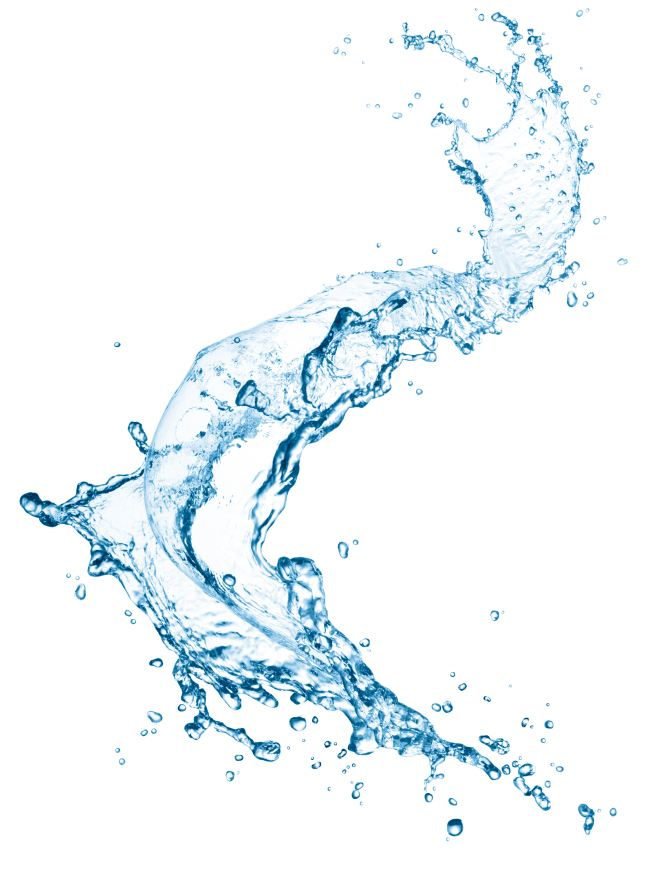
\includegraphics{figures/pic6.jpg}
        }
        %\includegraphics[scale=1.0]{figurefile}
        %\caption*{System components}
        \label{fig:system}
      \end{figure}
    \end{column}%
    \hfill%
    \begin{column}{.48\textwidth}
      \begin{itemize}
      \setbeamertemplate{itemize items}{\color{red}$\bullet$}  
        \item Texture-based method : minimize the calculation, wildly used in real time rendering
          \begin{itemize}
            \setbeamertemplate{items}[ball]  
            \item Blinn, 1978, Bump Mapping
          \end{itemize}
        \item Construction-based method : more mathematicall
          \begin{itemize}
            \setbeamertemplate{items}[ball]  
            \item Cosine function superposition algorithm
            \item Gerstner Wave
            \item B-spline
          \end{itemize}
      \end{itemize}
    \end{column}%
  \end{columns}
\end{frame}

\begin{frame}[t]{\emph{HOW} to simulate?}
  \textcolor[rgb]{0.5,0.5,0.5}{Quite difficult to deal with the \textbf{\color{blue}volatile} material...}
  \begin{columns} % align columns
    \begin{column}<0->{.48\textwidth}
      \begin{figure}[thpb]
        \centering
        \resizebox{0.8\linewidth}{!}{
        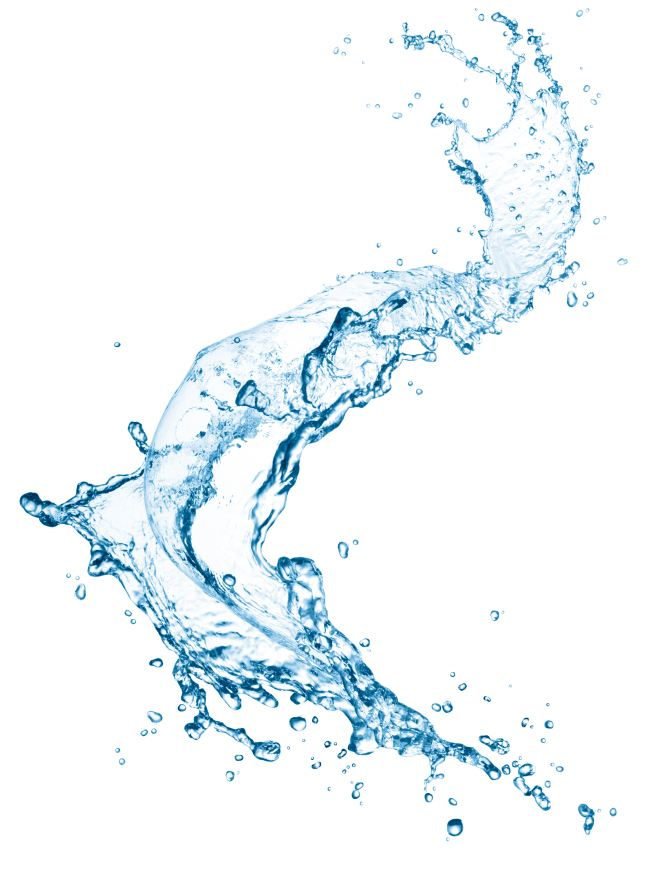
\includegraphics{figures/pic6.jpg}
        }
        %\includegraphics[scale=1.0]{figurefile}
        %\caption*{System components}
        \label{fig:system}
      \end{figure}
    \end{column}%
    \hfill%
    \begin{column}<0->{.58\textwidth}
      \\
      \begin{itemize}
      \setbeamertemplate{itemize items}{\color{red}$\bullet$}  
        \item Based on physics models : Realistic and Lifelike(pick it!\checkmark)
        \begin{figure}[thpb]
          \centering
          \resizebox{0.8\linewidth}{!}{
              \centering
              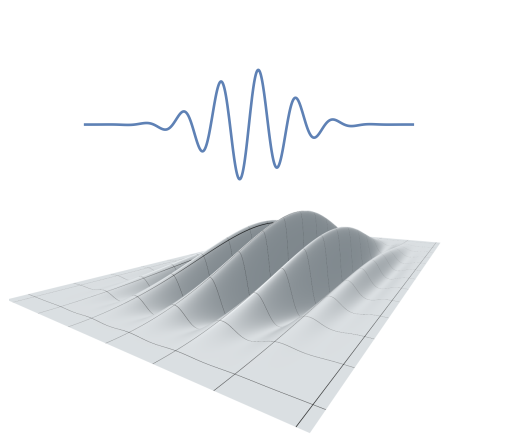
\includegraphics{figures/pic8.png}
          }
        \label{fig:system}
        \end{figure}
      \end{itemize}
    \end{column}%
  \end{columns}
\end{frame}




\begin{frame}{Introduction to Gerstner Wave}
  \begin{itemize}
    \item Wavelength (L)\\ 
    %the crest-to-crest distance between waves in world space. 
    %Wavelength L relates to frequency w as $w = 2/L$.
    \item Amplitude (A)\\
    %the height from the water plane to the wave crest.
    \item Speed (S)\\
    %the distance the crest moves forward per second. 
    %It is convenient to express speed as phase-constant phase-constant.jpg , where phase-constant.jpg = S x 2/L.
    \item Direction (D )\\
    %the horizontal vector perpendicular to the wave front 
    %along which the crest travels.
  \end{itemize}
  \begin{figure}[thpb]
    \centering
    \resizebox{0.6\linewidth}{!}{
        \centering
        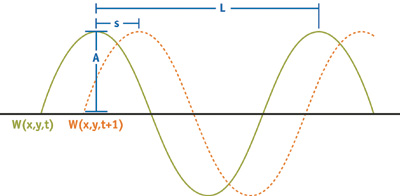
\includegraphics{figures/gerstner_intro.jpg}
    }
  \label{fig:gerstner_intro}
  \end{figure}
\end{frame}

\begin{frame}{Introduction to Gerstner Wave}
  对于单个波而言,其函数表达式如下所示。\\ 
  \begin{itemize}
    \item A 振幅 \\
    \item D 二维方向向量 \\
    \item w 角速度 \\
    \item $\varphi$ 其值为$S \times \frac{2}{L}$
  \end{itemize}
  $$W_i(x,y,t) = A_i \times \sin(D_i \cdot (x,y) \times w_i + t \times \varphi_i)$$
\end{frame}

\begin{frame}{Introduction to Gerstner Wave}
  完整的Gerstner Wave函数如下所示。其为向量值函数。
  \begin{itemize}
    \item 输入\\
      网格化的坐标值\\ 
    \item 输入 \\
      三维坐标系中的坐标(x, y, z) \\
  \end{itemize}
  $$
  P(x, y, t) = 
    \begin{pmatrix}
    x + \sum(Q_iA_i \times D_i[x] \times \cos(w_iD_i \cdot(x, y) + \varphi_it))\\
    y + \sum(Q_iA_i \times D_i[y] \times \cos(w_iD_i \cdot(x, y) + \varphi_it))\\
    \sum(A_i\sin(w_iD_i \cdot(x,y) + \varphi_i t))
    \end{pmatrix}
  $$
\end{frame}

\begin{frame}{参数特点}
  \begin{itemize}
    \item Q较大 \\
    波峰尖锐,类似于真实水面 \\
    \item Q过大 \\
    产生环,破坏波的形状 \\
    \item Q为0 \\ 
    退化为简单三角函数的叠加 \\
  \end{itemize}

  \begin{figure}[thpb]
    \centering
    \resizebox{1\linewidth}{!}{
        %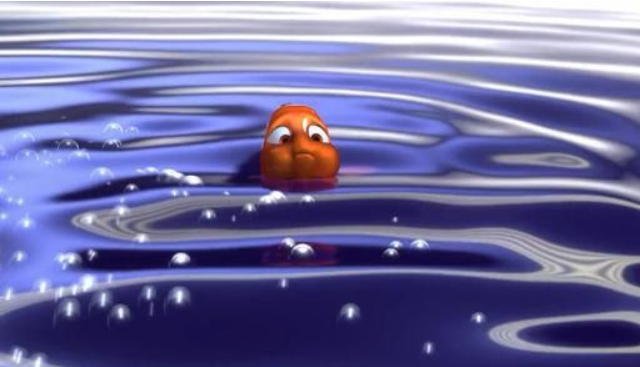
\includegraphics{figures/pic1.png}
        \begin{subfigure}[t]{0.5\textwidth}
        \centering
        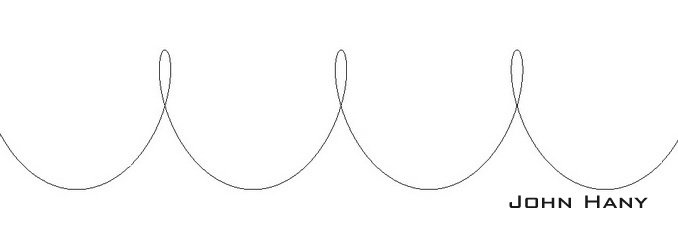
\includegraphics[width=1\textwidth]{figures/loop.jpg}
        \subcaption*{The first film}
        \end{subfigure}
        \quad
        \begin{subfigure}[t]{0.5\textwidth}
        \centering
        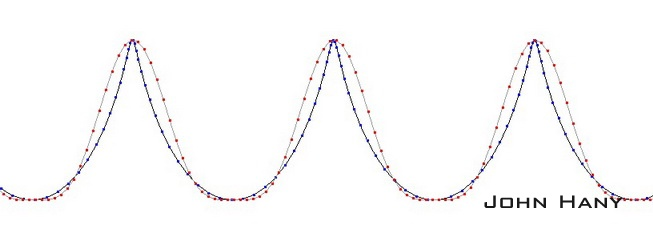
\includegraphics[width=1\textwidth]{figures/sharp.jpg}
        \subcaption*{The second film}
        \end{subfigure}
    }
    %\caption*{\emph{Finding Nemo}({\fangsong 海底总动员})}
  %\label{fig:1}
  \end{figure}
\end{frame}


\begin{frame}{Advantages}
  \begin{itemize}
    \item 波峰尖锐,波谷平缓
    \item 允许多波产生叠加效果,交互感真实
    \item 参数众多,可调节性强
    \item 性能较高,开销较小
  \end{itemize}
  \begin{figure}[thpb]
    \centering
    \resizebox{0.5\linewidth}{!}{
        \centering
        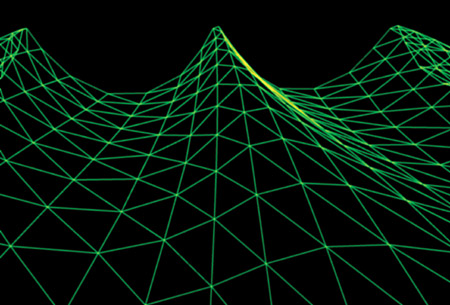
\includegraphics{figures/gerstner_dem.jpg}
    }
  \caption{Gerstner Wave}\label{fig:gerstner_dem}
  \end{figure}
\end{frame}

\begin{frame}{Disadvantaged}
  \begin{itemize}
    \item 水面永动,水面远处永远“自发地”泛起波纹
    \item 波峰低的波会产生大面积规律褶皱
    \item 无法仿真不同向的波间的碰撞和能量损耗。
        当波间相差的角度较大时,水面效果较差
    \item 整体上看,规律性过强
  \end{itemize}
\end{frame}


\begin{frame}{Refine}
  \begin{itemize}
    \item 波随机过滤\\
    对小波采取随机化地去除。
    \item 动态修改参数\\
    动态地略微地修改各个波的方向、振幅等参数。
  \end{itemize}

  \begin{figure}[thpb]
    \centering
    \resizebox{0.4\linewidth}{!}{
        \centering
        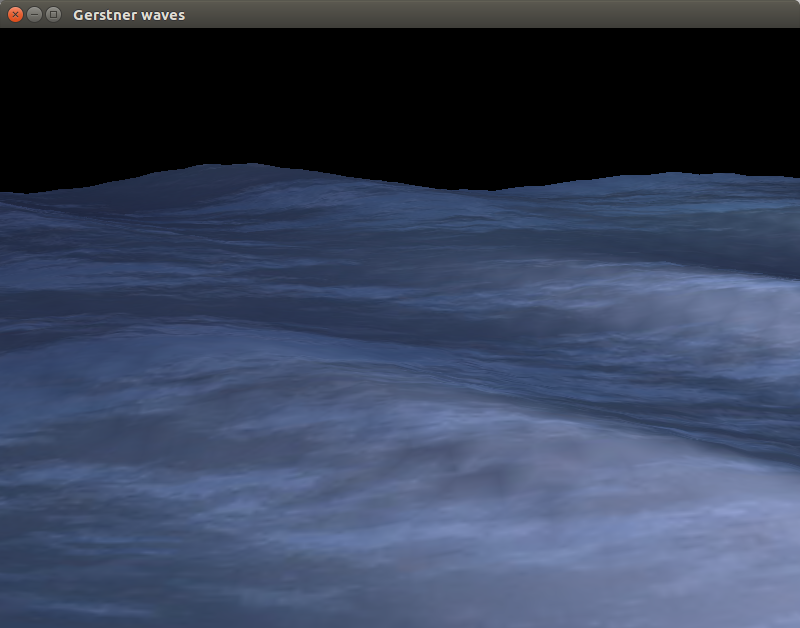
\includegraphics{figures/show.png}
    }
  \caption{程序运行图片}\label{fig:show}
  \end{figure}


\end{frame}




% % -----------------------------------------------------------------------------
% \section{Introducão}
% \begin{frame}{Introdução}
% %introducao
% A Introdução vai aqui
% \end{frame}
% %------------------------------------------------------------------------------

% %------------------------------------------------------------------------------
% \section{Referencial Teórico}
% \begin{frame}{Referencial Teórico}
% %referencial teorico, estado da arte, etc
% Referencial Teórico ou estado da arte.  
% \end{frame}
% %------------------------------------------------------------------------------

% %------------------------------------------------------------------------------
% \section{Metodologia}
% \begin{frame}{Metodologia}
% Metodologia minuciosamente aqui.
% \end{frame}
% %------------------------------------------------------------------------------

% %------------------------------------------------------------------------------
% \section{Considerações e Resultados}
% \begin{frame}{Considerações e Resultados}
% %consideraçoes e resultados
% Resultados e considerações do trabalho  
% \end{frame}
% %------------------------------------------------------------------------------

% %------------------------------------------------------------------------------
% \section{Referencias}
% \begin{frame}{Referencias}
%   Suas referencias bibliográficas aqui, siga o modelo ABNT.
% \end{frame}
% %------------------------------------------------------------------------------

% %------------------------------------------------------------------------------
% \section{Agradecimentos}
% \begin{frame}{Agradecimentos}
% Agradeço a todos que colaboraram  para realizaç~ao deste projeto.
% Agradeço ao Alexandre Bencz pelo assembly de cada dia.
% Agradeço ao Sonata Arctica, Avantasia, Mago de Oz, Cain's Offering, e todas as outras bandas de Power Metal. 	
% \end{frame}
% %------------------------------------------------------------------------------

% %------------------------------------------------------------------------------
% \subsection{Sites legais}
% \begin{frame}{Sites legais}
%   Want to know more? See!
%   \begin{itemize}
%     \item Browse in my page \url{http://www.ezefranca.com}.
%     \item Browse on BCC page \url{http://www.sp.sustech.br/bcc}.
%     \item Thanks WriteLaTeX from Support! \url{http://www.writelatex.com}.
%   \end{itemize}
  
% \end{frame}
% %------------------------------------------------------------------------------

% -----------------------------------------------------------------------------
\end{document}
%-----------------------------------------------Este comentario nunca aparecera